%%%%%%%%%%%%%%%%%%%%%%%%%%%%%%%%%%%%%%%%%%%%%%%%%%%%%%%
% A template for Wiley article submissions.
% Developed by Overleaf. 
%
% Please note that whilst this template provides a 
% preview of the typeset manuscript for submission, it 
% will not necessarily be the final publication layout.
%
% Usage notes:
% The "blind" option will make anonymous all author, affiliation, correspondence and funding information.
% Use "num-refs" option for numerical citation and references style.
% Use "alpha-refs" option for author-year citation and references style.

\documentclass[alpha-refs]{wiley-article}
% \documentclass[blind,num-refs]{wiley-article}

% Add additional packages here if required 
\usepackage{siunitx}

\newcommand{\sahir}[1]{\textcolor{red}{#1}}
% Update article type if known
\papertype{Original Article}
% Include section in journal if known, otherwise delete
\paperfield{Significance}

\title{Speed kills ; slowing the spread of COVID-19 saves lives}

% List abbreviations here, if any. Please note that it is preferred that abbreviations be defined at the first instance they appear in the text, rather than creating an abbreviations list.
%\abbrevs{ABC, a black cat; DEF, doesn't ever fret; GHI, goes home immediately.}

% Include full author names and degrees, when required by the journal.
% Use the \authfn to add symbols for additional footnotes and present addresses, if any. Usually start with 1 for notes about author contributions; then continuing with 2 etc if any author has a different present address.
\author[1,2]{Luke Anderson-Trocm\'e}
\author[2,3]{Sahir Bhatnagar}
%\author[2\authfn{2}]{Author Three PhD}
%\author[2]{Author B.~Four}

%\contrib[\authfn{1}]{Equally contributing authors.}

% Include full affiliation details for all authors
\affil[1]{Department of Human Genetics, McGill University, Montreal, QC H3A 0G1, Canada}
\affil[2]{McGill University and Genome Quebec Innovation Centre, Montreal, QC H3A 0G1, Canada}
\affil[3]{Department of Epidemiology, Biostatistics and Occupational Health, McGill University, Montreal, QC H3A 0G1, Canada}

%\corraddress{Sahir Bhatnagar, Department of Epidemiology, Biostatistics and Occupational Health,  McGill University, Montreal, QC H3A 0G1, Canada}
%\corremail{sahir.bhatnagar@mcgill.ca}

%\presentadd[\authfn{2}]{Department, Institution, City, State or Province, Postal Code, Country}

%\fundinginfo{Funder One, Funder One Department, Grant/Award Number: 123456, 123457 and 123458; Funder Two, Funder Two Department, Grant/Award Number: 123459}

% Include the name of the author that should appear in the running header
\runningauthor{Anderson-Trocm\'e \& Bhatnagar}

\begin{document}

\maketitle
\begin{abstract}
As the Novel Coronavirus pandemic continues to spread around the globe, scientists and politicians alike are scrambling to develop policies to limit the spread of the virus and \textit{flatten the curve}.
While some outbreaks appear to have passed their peaks allowing for a gradual return to normalcy, others are still bracing for the peak to come.
Guidelines about how and when social distancing measures can be lifted are dependent on limiting the  the spread of the virus to a manageable rate to avoid surging hospital capacities.
%These differences from region to region beg the question : how do these outbreaks compare to one another?
%However, the exponential nature of viral outbreaks make it difficult to visualize these differences in an intuitive manner.
Here we argue that the doubling time of case counts is a more intuitive metric to use for evaluating the management of coronavirus outbreaks around the world.

%This is a generic template designed for use by multiple journals, which includes several options for customization. Please consult the author guidelines for the journal to which you are submitting in order to confirm that your manuscript will comply with the journal's requirements. Please replace this text with your abstract.

% Please include a maximum of seven keywords
\keywords{coronavirus, COVID-19, pandemic, \emph{doubling time}, log ratio}
\end{abstract}


\section{Introduction}

%\subsection{A novel viral outbreak}
%%rejected sentences
%impacted the lives of nearly everyone as social distancing measures have rapidly become the norm.

The Novel Coronavirus pandemic was first reported in December 2019; as it spreads across the globe and testing protocols capture the rapidly increasing case counts, a number of countries have implemented new policies to help mitigate the spread of this virus.
The number of COVID-19 cases from outbreak to outbreak varies as a result of a number of factors like population density, arrival time of the first cases, the variability in \textit{pandemic preparedness} and the timing and nature of government responses.
The discrepancies between COVID-19 case counts has been subject to a number of reports comparing countries and \textit{how well} they are handling the outbreak.
However, there are many confounding factors that make it difficult to compare outbreaks based solely on case counts.
In this article, we discuss critical limitations when comparing data between countries and propose the use of the \textit{speed} of spread as a better alternative to case counts when monitoring the progress of outbreaks.

%The transmission rate of the virus in each region can be modelled based on the features of a defined host environment like the timing of the implementation of social distancing policies, the  population density and ...

\begin{figure}[bt]
\centering
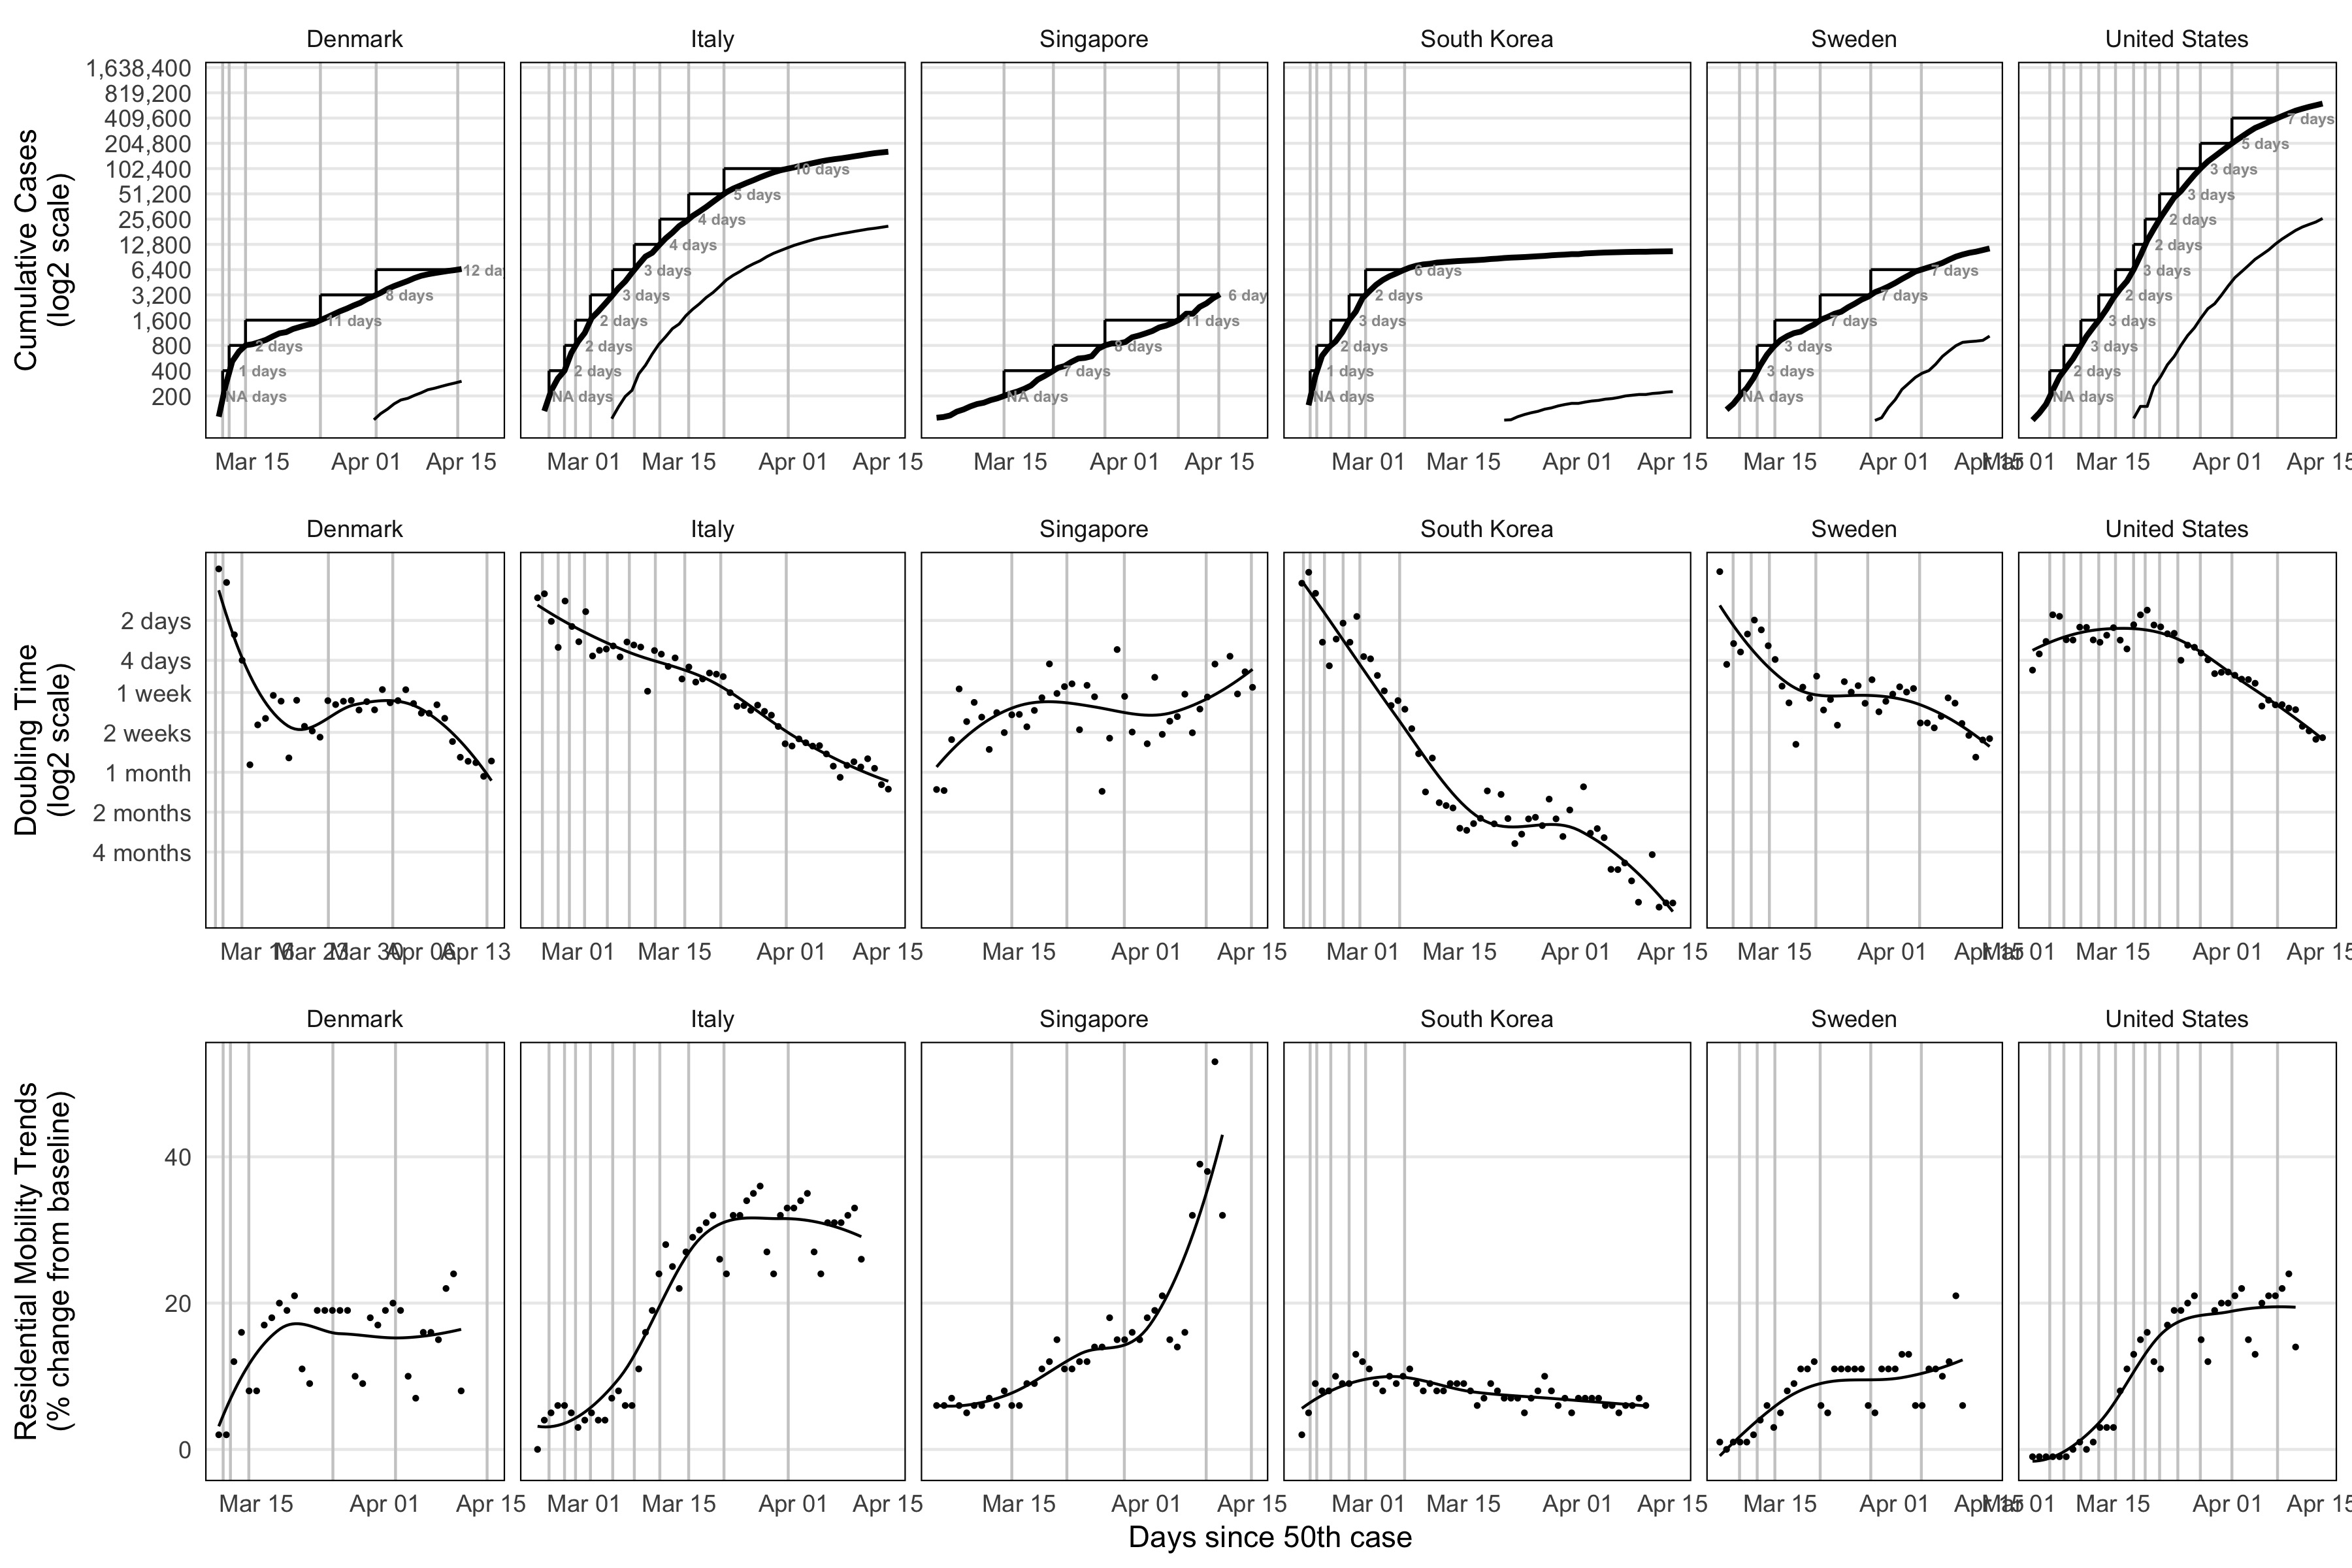
\includegraphics[width=\hsize,keepaspectratio]{doubling_time_select6.jpg}
\caption{
Comparing the rate of spread of COVID-19 cases in six countries.
\textbf{Top row :}  
The \textit{dashed line} is the cumulative number of tests, the \textit{solid line} is the cumulative number of confirmed COVID-19 cases and the \textit{dotted} line is the cumulative number of reported deaths related to COVID-19.
The grid lines correspond to instances of doubling of case counts where the number on top of the tick is the time it took for each doubling. 
To illustrate this, we highlight the time it takes (x axis) to reach another doubling instance (y axis).
Pandemic mitigation policy implementation are marked as yellow dots.
\textbf{Middle row :}  
The doubling time of confirmed cases of COVID-19. Larger doubling times indicate a reduction in the speed of the spread of the virus.
\textbf{Bottom row :}  
The percent change in residential mobility trends from Google Mobility Report. 
While comparing mobility trends between countries has its limitations, the alignment of the reduction in the speed of spread and the increase in people staying home is notable.
}
%Although we encourage authors to send us the highest-quality figures possible, for peer-review purposes we are can accept a wide variety of formats, sizes, and resolutions. Legends should be concise but comprehensive ? the figure and its legend must be understandable without reference to the text. Include definitions of any symbols used and define/explain all abbreviations and units of measurement.}
\label{doub_time}
\end{figure}

\section{Visualizing the curve}

%One of the most referenced infectious disease models of the Novel Coronavirus came from Imperial College London which raised awareness on the dangers of inaction by modelling the spread of the virus in the United Kingdom and the United States.
%They estimated mass death if no mitigation action was to be taken and drastic decreases in mortality if mitigation measures were taken.
As case counts began to grow, so did the talk of \textit{flattening the curve}.
This catch phrase summarizes the goal of pandemic mitigation policies : limiting the number of people who are simultaneously infected can avoid exhausting the capacity of health care systems which in turn leads to more lives saved.
However common the phrase may be, it begs the question : What \textit{curve} are we trying to flatten? And what do these \textit{curves} tell us about where we're headed?

Any data visualization has its limitations --- including those presented here. 
We need to critically think about these graphs and be careful not to arrive at hasty conclusions, particularly when it comes to comparing the performance of countries during this pandemic. 
Media and politicians are too quick to compare the total number of infections and claim victory because theirs are ``lower'' than others. This is problematic for many reasons and can lead to premature re-opening of society.


One of the most common visualizations comparing outbreaks is the cumulative number of people who have tested positive for the Novel Coronavirus.
However, cumulative case counts can be misleading for a number of reasons.
First, these counts don't account for population size. 
Per-capita case counts seem like a good alternative, however especially in the early stages of an infectious disease outbreak, countries with small population sizes will have disproportionately larger values. In short time periods, where we can assume the population size doesn't change, per-capita adjusted curves will only be shifted up or down. Their \textit{shape} doesn't change.
Second, the exponential nature of viral outbreaks makes it difficult to compare the scales of outbreaks between regions.
Is a log10 scale better than a log2 scale?
Logarithmic scales are difficult to decipher visually, especially for a lay audience.
Thirdly, most references to a proverbial peak of the curve are really referring to the change in the rate of the spread.
Small fluctuations in the rate of change are difficult to see on logarithmic scales let alone comparing these across regions.

\subsection{Doubling time}

We argue that a more natural comparison between outbreaks lies in the change of the rate of spread itself.
Rather than rely on the daily raw counts of positive cases which are difficult to interpret, changes in the speed of spread are more easily interpreted.
One outbreak may be spreading twice as fast as another outbreak despite having fewer total infections.


The rate of spread is also a more "real time" estimation of how the virus is spreading in the population.
This is most evident when comparing the doubling time to Google's Mobility Reports (Figure \ref{doub_time} C).
An increase in residential activity (or people staying home) directly follows the implementation of social distancing policies.
These distancing measures then lead to a drop in the rate of spread of the virus.

\begin{figure}[bt]
\centering
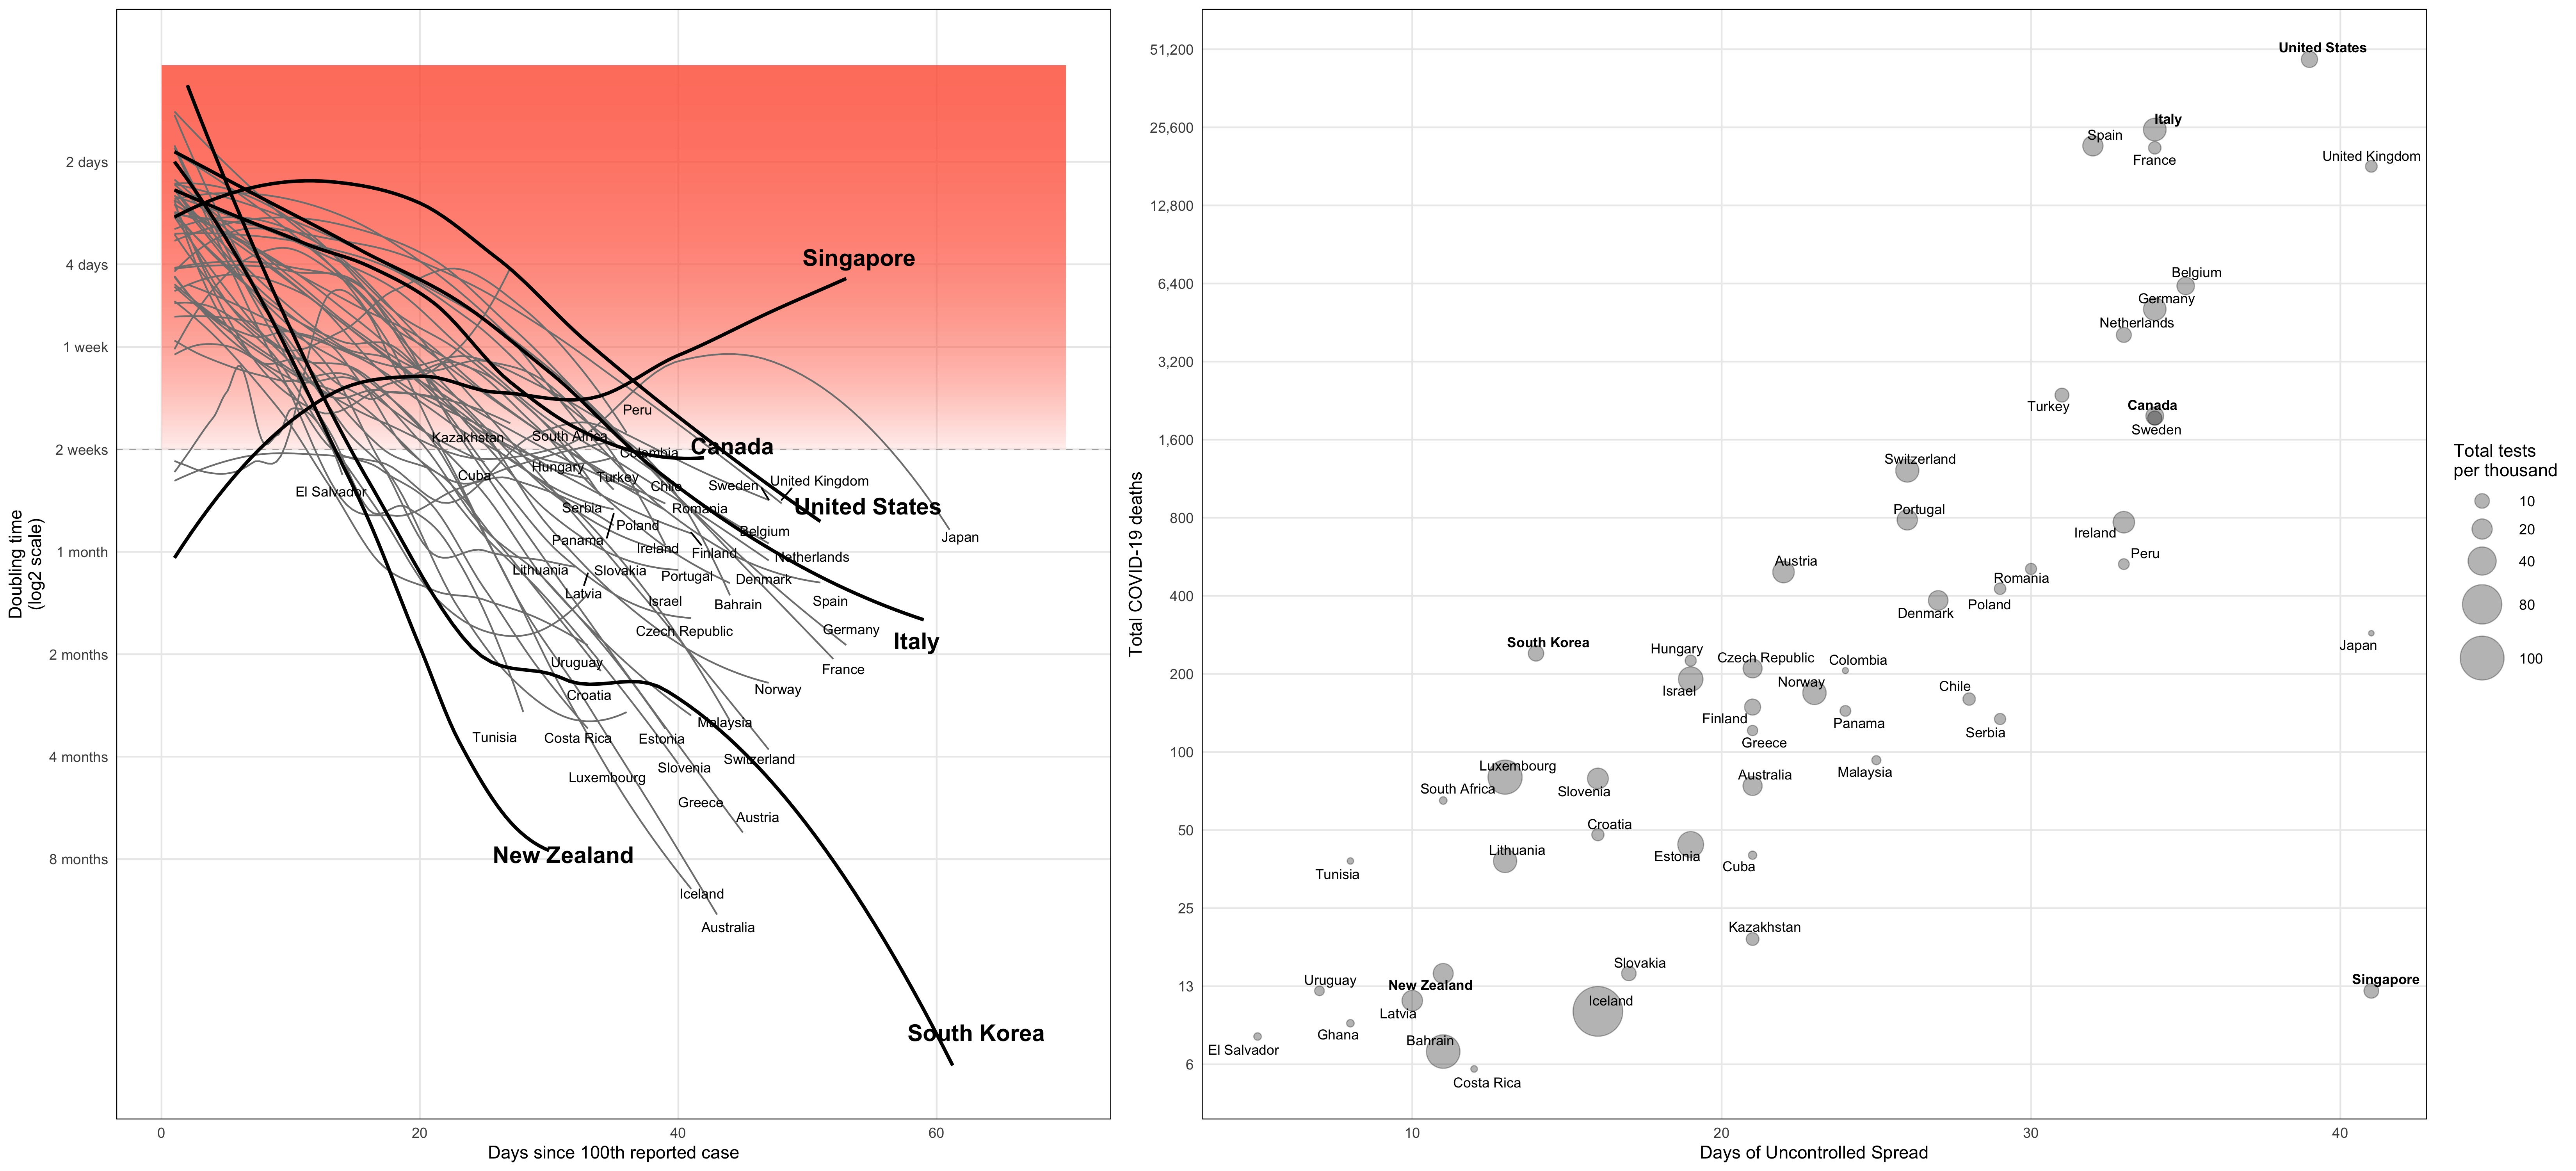
\includegraphics[width=\hsize,keepaspectratio]{time_to.jpg}
\caption{
Flattening the curve rapidly saves lives.
\textbf{Left  :} Comparing the doubling time of COVID-19 cases between countries.
\textbf{Rigt  :} Countries that manages to reduce the spread of the virus quickly have fewer COVID-19 related deaths. The size of the circles is proportional to the number of covid tests per 10000 individuals.
}
\label{time}
\end{figure}

\subsection{Reaction time}
Social distancing measures tend to reduce the rate of spread of the virus.
A reduction in contact between people will limit the number of transmissions and thus reduce the number of new infections.
Comparing the effectiveness of mitigation measures between outbreaks is difficult as many variables like population density, testing capacities and contact tracing also vary from region to region.
This being said, the timing of the implementation of such policies does appear to have an impact on the severity of the outbreak.
When social distancing policies are implemented rapidly, the spread of the virus decreases more rapidly which correlates strongly with lower mortality.
Conversely, slower responses allow the virus to spread freely for longer leading to exponentially more infections.
These rapid increases in case counts lead to surges in hospitalizations with limited hospital capacities.

\subsection{Opening up too early can do more harm than good}
Countries like Japan and Singapore were touted as early success stories for limiting the spread of the virus. 
However, both of these countries have seen recent increases in cases that can only be described as the onset of a second wave of COVID-19 cases.
While the reasons for how the second waves are unknown, one thing we can tell is the doubling time of cases in both these countries show a real time response.
%Lessons can be learned, we can use this as a speedometer.
%Using doubling time as a speedometer. 

\subsection{Apples and oranges}
Differences in data collection across different countries can impact our ability to compare outbreaks.
For example, a country that only tests highly suspect cases will have a lower case count than a country that tests all suspected cases.
This could also impact the measured mortality rate of the virus as outbreaks that limit testing to severe outcomes will inherently have a much higher mortality rate than a country that captures the less severe cases as well.
Moreover, some countries have only released hospitalized COVID-19 related deaths while others have been including COVID-19 related deaths from retirement homes.
%It is understandable that many of these non-hospitalized deaths are more difficult to confirm as COVID-19 related deaths and thus may take longer to release to the public. 



\section{Conclusion}



\sahir{This conclusion sounds out of place. I think the sticking points should be centered around} 
\begin{enumerate}
    \item \sahir{rates of change as a natural metric everyone can understand compared to cumulative counts. }
\item \sahir{Difficulty in comparing countries because of a variety of factors you've mentioned.} 
\item \sahir{A more comprehensive look at the data simultaneously (e.g. tests, doubling time, deaths) can mitigate some of the issues mentioned in 2)}
\item \sahir{There are still limitations with every graph, including the ones presented here. We need to critically think about each one and be careful not to arrive at hasty conclusions, particularly when it comes to comparing the performance of countries during this pandemic. Media and politicians are too quick to look at cumulative curves between countries and claim victory because they are ``lower'' than the other. This is problematic for many reasons and can lead to premature re-opening of society. In light of this (RE: your title about speed kills), I would actually say that misinformation kills!}
\end{enumerate}



\section*{acknowledgements}
We would like to thank (people who helped) for their conversations as well as (data resources) for their help in making the data used available to us.
%Acknowledgements should include contributions from anyone who does not meet the criteria for authorship (for example, to recognize contributions from people who provided technical help, collation of data, writing assistance, acquisition of funding, or a department chairperson who provided general support), as well as any funding or other support information.

\bibliography{sample}

\end{document}
